\section{Selected Results on Alignment of the Tracking System with~2015 Data}
\label{sec:alignmentResults}

Different data-taking periods in 2015 include periods of cosmic ray data-taking with the magnetic field $B=0$T and $B=3.8$T, and periods of collision data-taking at $\sqrt{s}=13$~TeV center-of-mass energy with $B=0$T and $B=3.8$T. Different data-taking periods correspond to different detector geometries particularly due to changes of the magnetic field. 

% (1) MY WORDS:
Alignment constants were derived separately for each of the data-taking periods using the alignment results of the previous period of data-taking as a starting point. Millepede-II and HIP algorithms were run in sequence to perform the alignment, as well as two algorithms, were run independently for cross checking. 

% (2) NO PLAGIARISM 
The first alignment of the tracker corrected for the displacements that took place between the Run~I and Run~II. Cosmic ray data with magnetic field turned on ($B=3.8$T) and off ($B=0$T) were used for this alignment. The modules in certain parts of BPIX were repaired during the shutdown, and all pixel subdetectors were moved within the tracker. 

After the cosmic ray data taking periods, the magnetic field was turned off again, and the first collisions were detected with $B=0$T. This change in the magnetic field caused movements in the tracking system that has the strongest effect in the pixel subdetectors. The alignment performed using~$B=0$T collisions and cosmic ray data recovers the tracker performance in the ability to reconstruct kinematic parameters of charged particles. When the magnetic field was turned back on, the large substructures of BPIX and FPIX have displaced again, and, thus, the tracking system was aligned again to recover these displacements.  

% (3) MY WORDS
Validation of tracking system alignment tools include geometry comparison tool (Ch.~\ref{sec:AlRes_GCP}), validation using distribution of median residuals (Ch.~\ref{sec:AlRes_DMRs}), cosmic track splitting validation (Ch.~\ref{sec:AlRes_trackSplit}), and primary vertex validation (Ch.~\ref{sec:AlRes_PVvalid}). Full results of the first alignment with Run~II data are available at~\cite{ref_AlApproved_twiki}.

\subsection{Geometry Comparison}
\label{sec:AlRes_GCP}

% (4) MY WORDS:
Geometry comparison visualizes differences in positions of modules between two different geometries of the CMS tracking system. Figure~\ref{fig:GCP_FPIX} shows the comparison between positions of the FPIX modules between Run~I and Run~II geometries. Each dot in the figure corresponds to one module. Four clusters of red dots (Fig.~\ref{fig:GCP_FPIX}, left) and shifted parts at ($\phi<-\pi/2$, $\phi>\pi/2$) and ($-\pi/2<\phi<\pi/2$) (Fig.~\ref{fig:GCP_FPIX}, right) represent displacements of four half-disks by~4.5 and~5.5~mm at the $-z$ side of the FPIX. At the $+z$ side of the FPIX small relative movements of individual modules are observed only. For more intuitive visualization, the three-dimensional plot of the pixel detector is produced (Fig.~\ref{fig:GCP_3D}).     

\begin{figure}[htb]
    \begin{center}
        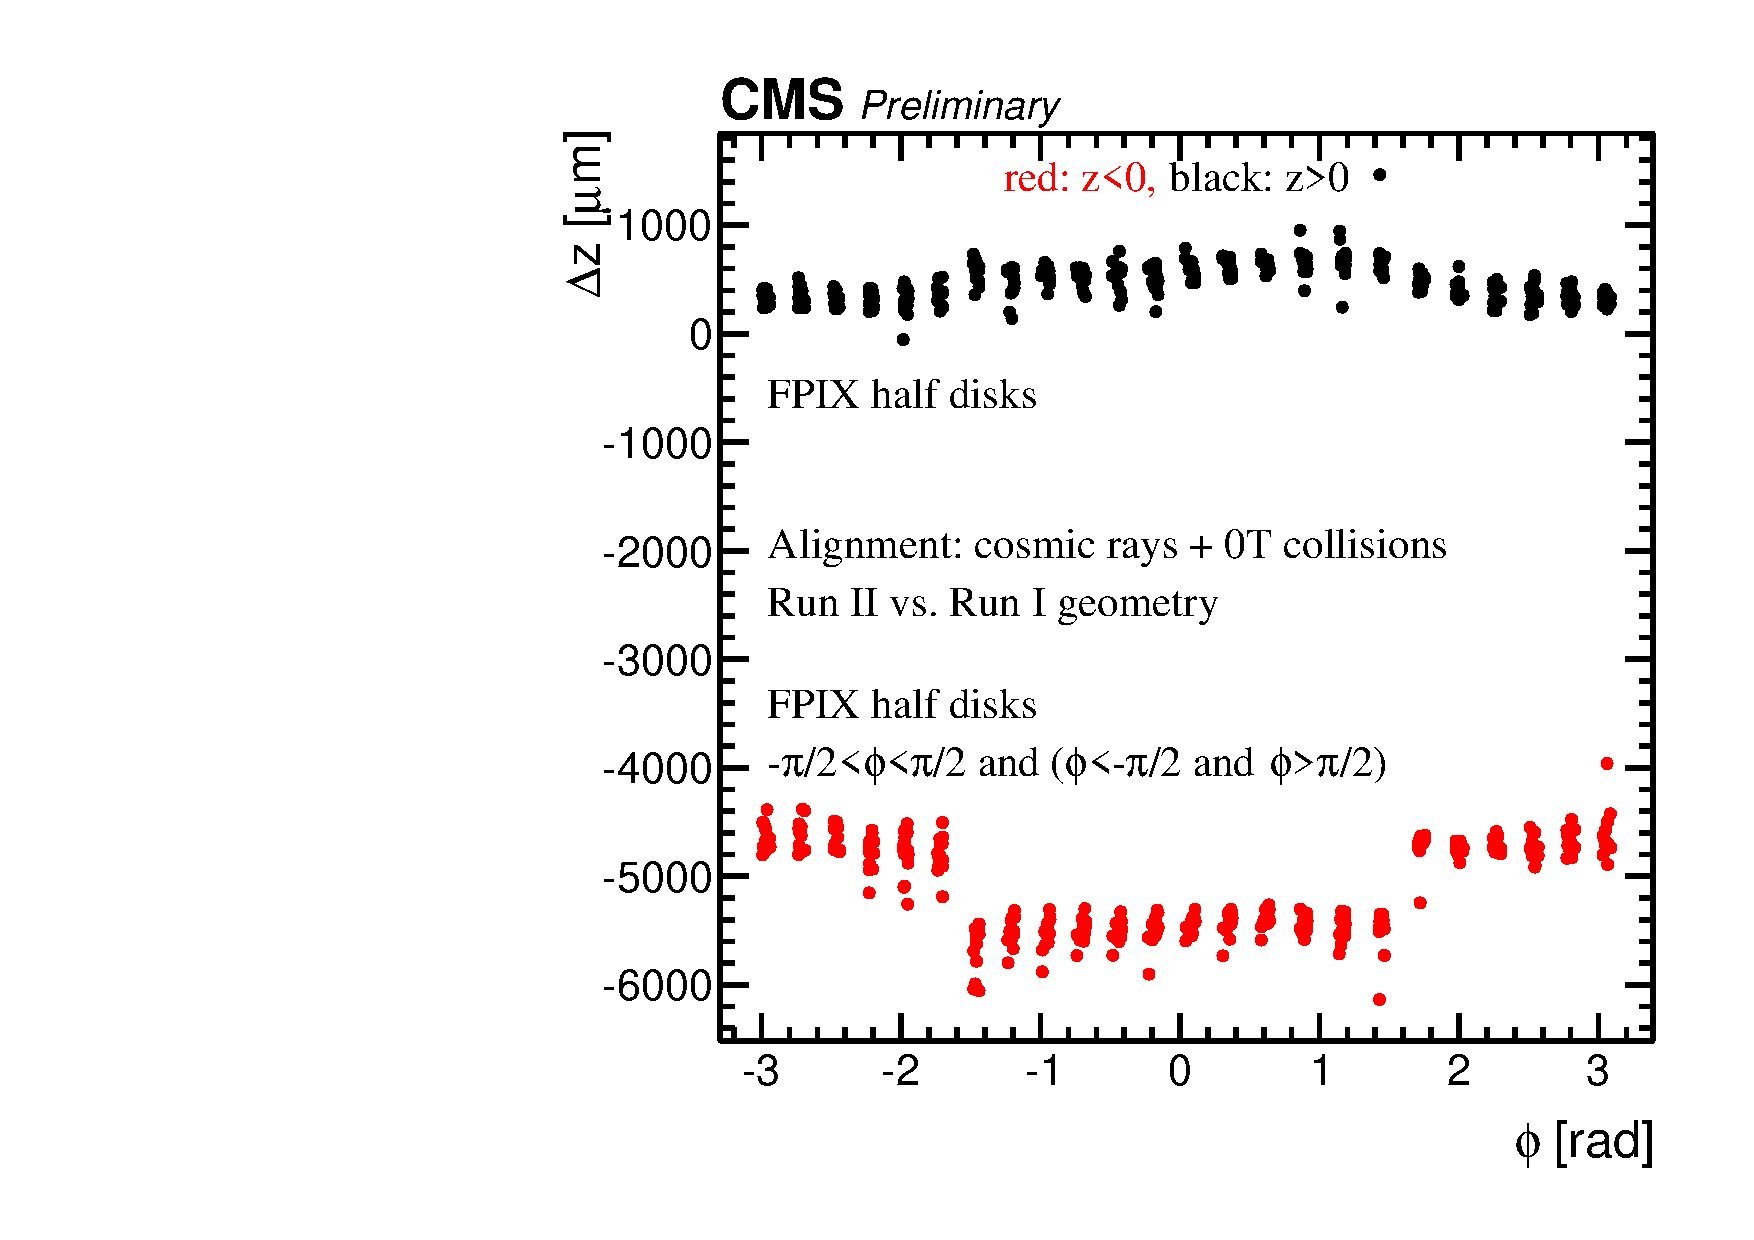
\includegraphics[width=0.45\textwidth]{../figs/Alignment/AlRes_phi_vs_dz_PXF_1.pdf}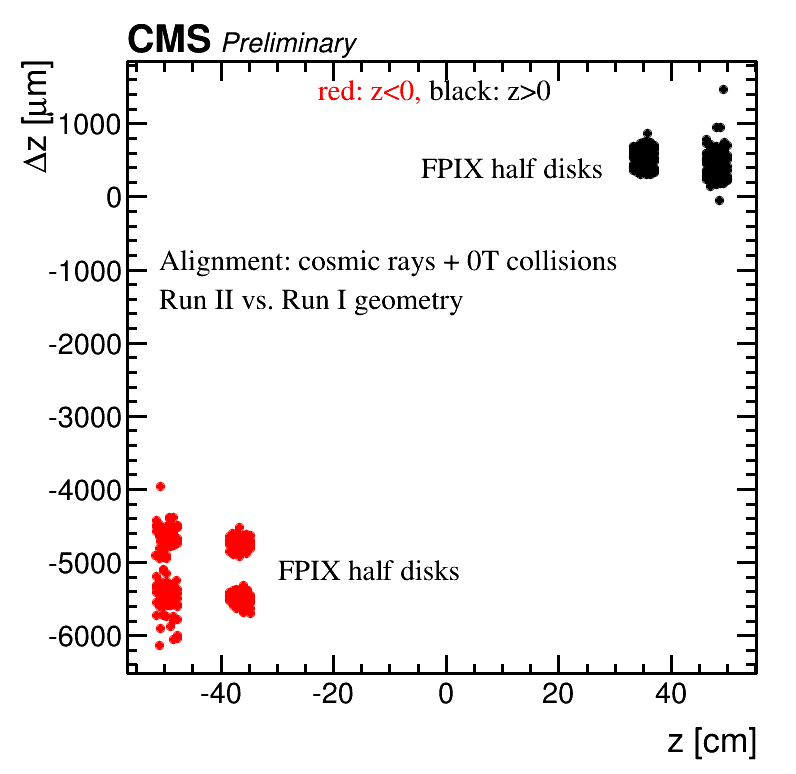
\includegraphics[width=0.45\textwidth]{../figs/Alignment/AlRes_z_vs_dz_PXF_1.png}
    \end{center}
    \caption{Comparison of Run~II and Run~I positions of the modules in the FPIX of the CMS tracking system. Positions are determined with the Millepede-II and HIP algorithms using cosmic ray data collected with the magnetic field of $B=0$T and $B=3.8$T magnetic field in the CMS solenoid. The difference $\Delta z$ (Run~II~-~Run~I) is plotted as a function of $z$ (left) and $\phi$ (right) in global coordinates.}
    \label{fig:GCP_FPIX}
\end{figure}

\begin{figure}[htb]
    \begin{center}
        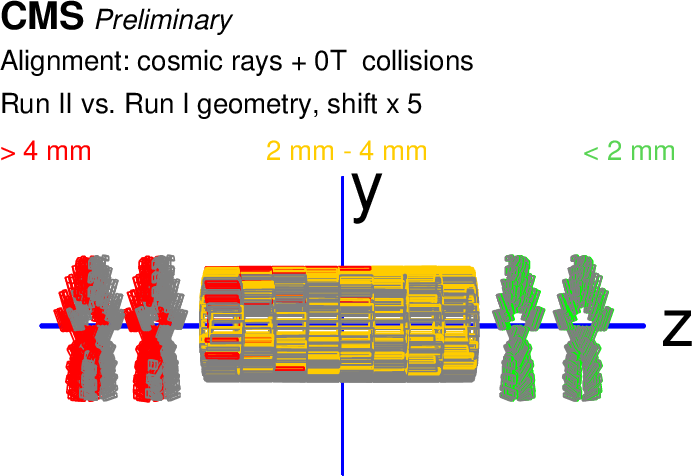
\includegraphics[width=0.95\textwidth]{../figs/Alignment/AlRes_RunIIvsRunI.png}
    \end{center}
    \caption{Three-dimensional geometry comparison of Run~II and Run~I positions in the BPIX and FPIX of the CMS tracking system. Positions are determined with the Millepede-II and HIP algorithms using cosmic ray data collected with the magnetic field of $B=0$T and $B=3.8$T magnetic field in the CMS solenoid and collision data with $B=0$T at $\sqrt{s}=13$~TeV. The positions at the end of Run~I are shown in gray. The module displacements between Run~I and Run~II are magnified by a factor of~5 for visualization purpose. The resulting positions are shown in red, yellow, or green, depending on the displacement magnitude. }
    \label{fig:GCP_3D}
\end{figure}

\subsection{Distributions of Medians of Unbiased Track-Hit Residuals}
\label{sec:AlRes_DMRs}

%(5) ALMOST QUOTE:
% Besides geometry comparison, we also have distributions of medians of unbiased track-hit residuals (DMR) validation tool. Each track is refitted using the alignment constants under consideration, and the hit prediction for each module is obtained from all of the other track hits. The median of the distribution of unbiased hit residuals is then taken for each module and is histogrammed. The width of this DMR is a measure of the statistical precision of alignment results; deviations from zero indicate possible biases. The width also has an intrinsic component due to the limited number of tracks, meaning that distributions can only be compared if they are produced with the same number of tracks, as is the case within each set of plots here. 
% (5) MY WORDS:
Besides geometry comparison, we also have distributions of medians of unbiased track-hit residuals (DMR) validation tool. Each track from a given dataset is refitted using prepared alignment constants, and the hit for each module is predicted from all other hits of the track. After that, DMRs of all modules in a given subdetector are plotted on the same histogram. The width of the prepared DMR is a measure of the statistical precision of the derived alignment results. 

%(6) NO PLAGIARISM DETECTED
%The DMRs in the transverse and longitudinal planes are studied in bins of track azimuth angle $\phi$ and pseudorapidity $\eta$. Random misalignments of the modules affect only the resolution of the unbiased track-vertex residual, increasing the width of the distributions, but without biasing their mean. Systematic movements of the modules will bias the distributions in a way that depends on the nature and size of the misalignment and the and of the selected tracks.

% (7) NO PLAGIARISM DETECTED
The DMRs are plotted for the local $x$- (Fig.~\ref{fig:DMRs}, left) and $y$-directions (Fig.~\ref{fig:DMRs}, right) in the BPIX. The blue line shows the DMR for Run~I while the green line shows the aligned geometry. The RMS values show that performance of the aligned geometry is improved by a factor of~10 over the Run~I geometry.

\begin{figure}[htb]
    \begin{center}
        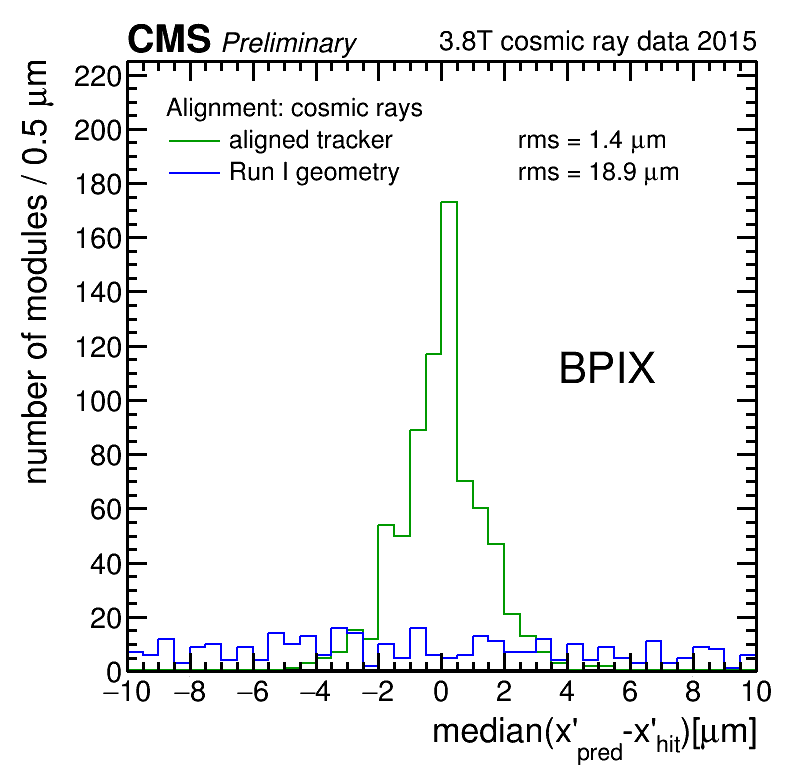
\includegraphics[width=0.45\textwidth]{../figs/Alignment/AlRes_CRAFT_DmedianR_BPIX_plain.png}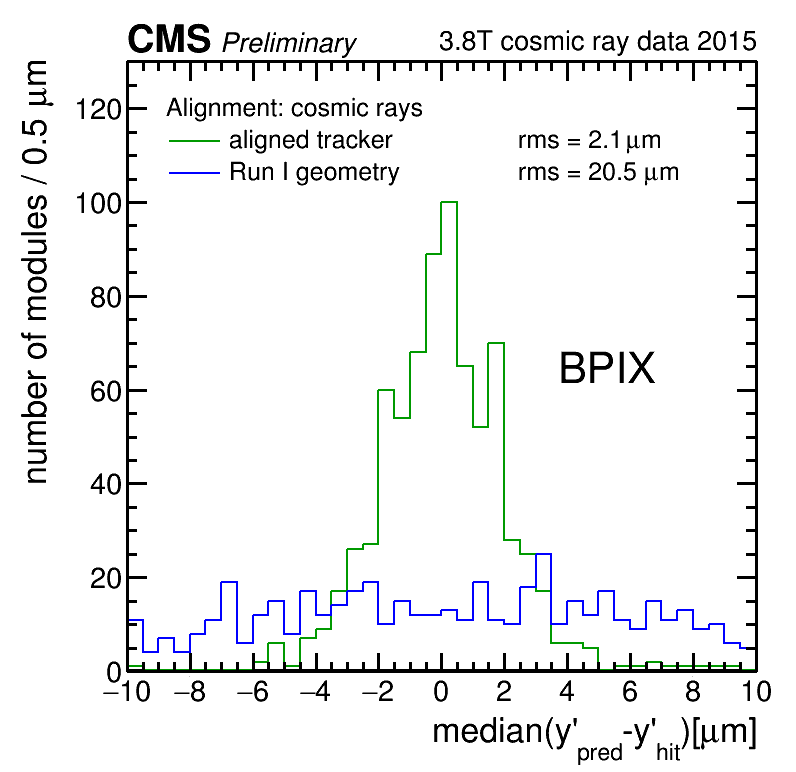
\includegraphics[width=0.45\textwidth]{../figs/Alignment/AlRes_CRAFT_DmedianYR_BPIX_plain.png}
    \end{center}
    \caption {DMRs for the local $x$-direction (left) and for the local $y$-direction (right) in the BPIX of the CMS tracking system, using~2 million cosmic ray tracks collected with the magnetic field of $B=3.8$T. The blue line shows the Run~I geometry. The green line shows the alignment produced with the Millepede-II and HIP algorithms using cosmic ray data at $B=0$T and $B=3.8$T.}
    \label{fig:DMRs}
\end{figure}

\subsection{Cosmic Track Splitting Validation}
\label{sec:AlRes_trackSplit}

% (8) ALMOST QUOTE
%Cosmic ray tracks are split in half at the hit closest to origin and refitted with the alignment constants under consideration. The differences in various track parameters between the two half-tracks are studied. The width of the distribution measures the achieved alignment precision, while deviations from zero indicate possible biases. 
%Results of the cosmic track splitting validation are shown in Fig.~\ref{fig:trackSplit}. The normalized differences between two halves of a cosmic track, split at the point of closest approach to the interaction region, in $d_{xy}$ (Fig.~\ref{fig:trackSplit}, left), the $xy$ distance between the track and the origin, and in $d_z$ (right), the distance in the $z$ direction between the track and the origin. The observed precision using the aligned geometry (green circles), produced with the Millepede-II and HIP algorithms using cosmic ray data at $B=0$T and $B=3.8$T, is a major improvement over the Run~I geometry (blue empty squares). The precision comes close to that of the ideal Monte Carlo, illustrating that the tracker has almost reached its design spatial resolution.
% (8) MY WORDS:
To perform the cosmic track splitting validation, cosmic tracks are split into two parts at the hit closest to the center of the detector and both parts are reconstructed separately using alignment results. After that, the distributions of the differences in track parameters are prepared. The RMS values of the distributions are measures of the precision of the alignment constants. A deviation of a central value from zero would indicate a bias. The results of this validation for~2015 alignment are shown in Fig.~\ref{fig:trackSplit}.

\begin{figure}[htb]
    \begin{center}
        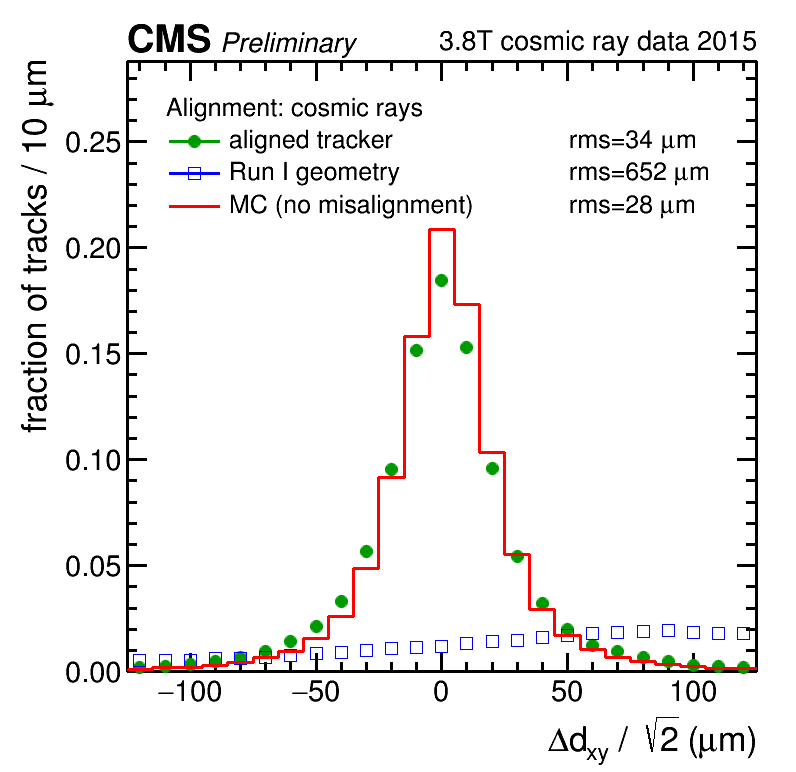
\includegraphics[width=0.45\textwidth]{../figs/Alignment/AlRes_CRAFT_hist_Delta_dxy.png}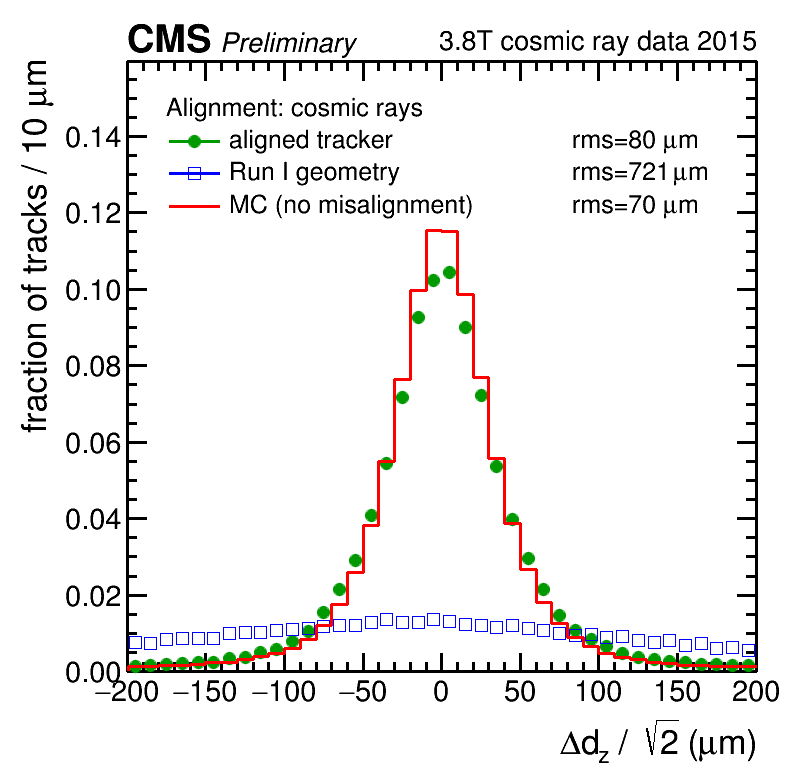
\includegraphics[width=0.45\textwidth]{../figs/Alignment/AlRes_CRAFT_hist_Delta_dz.png}
    \end{center}
    \caption{Results of the cosmic track splitting validation. The normalized differences between two parts of a cosmic track in the $xy$ distance between the track and the origin ($d_{xy}$, left), and in the distance in the $z$ direction between the track and the origin ($d_z$, right). Alignment is produced with the Millepede-II and HIP algorithms using cosmic ray data at the magnetic field of $B=0$T and~$B=3.8$T of CMS solenoid. Aligned geometry is shown in green.}
    \label{fig:trackSplit}
\end{figure}

\subsection{Primary Vertex Validation}
\label{sec:AlRes_PVvalid}

% (10) NO PLAGIARISM DETECTED
The resolution of the reconstructed vertex position is driven by the pixel subdetectors as the closest subdetectors to the interaction point which also have the best hit resolution. The primary vertex validation is based on the study the distances between tracks and the reconstructed vertex. 

%(11) NO PLAGIARISM DETECTED
Figure~\ref{fig:PVvalidation} compares the previous alignment to the one of a previous alignment reached during the commissioning phase with cosmic ray tracks at full magnetic field and to a detailed detector simulation with perfect alignment and calibration. The structures of the green curve indicate relative movements of the pixel half-barrels.

\begin{figure}[htb]
    \begin{center}
        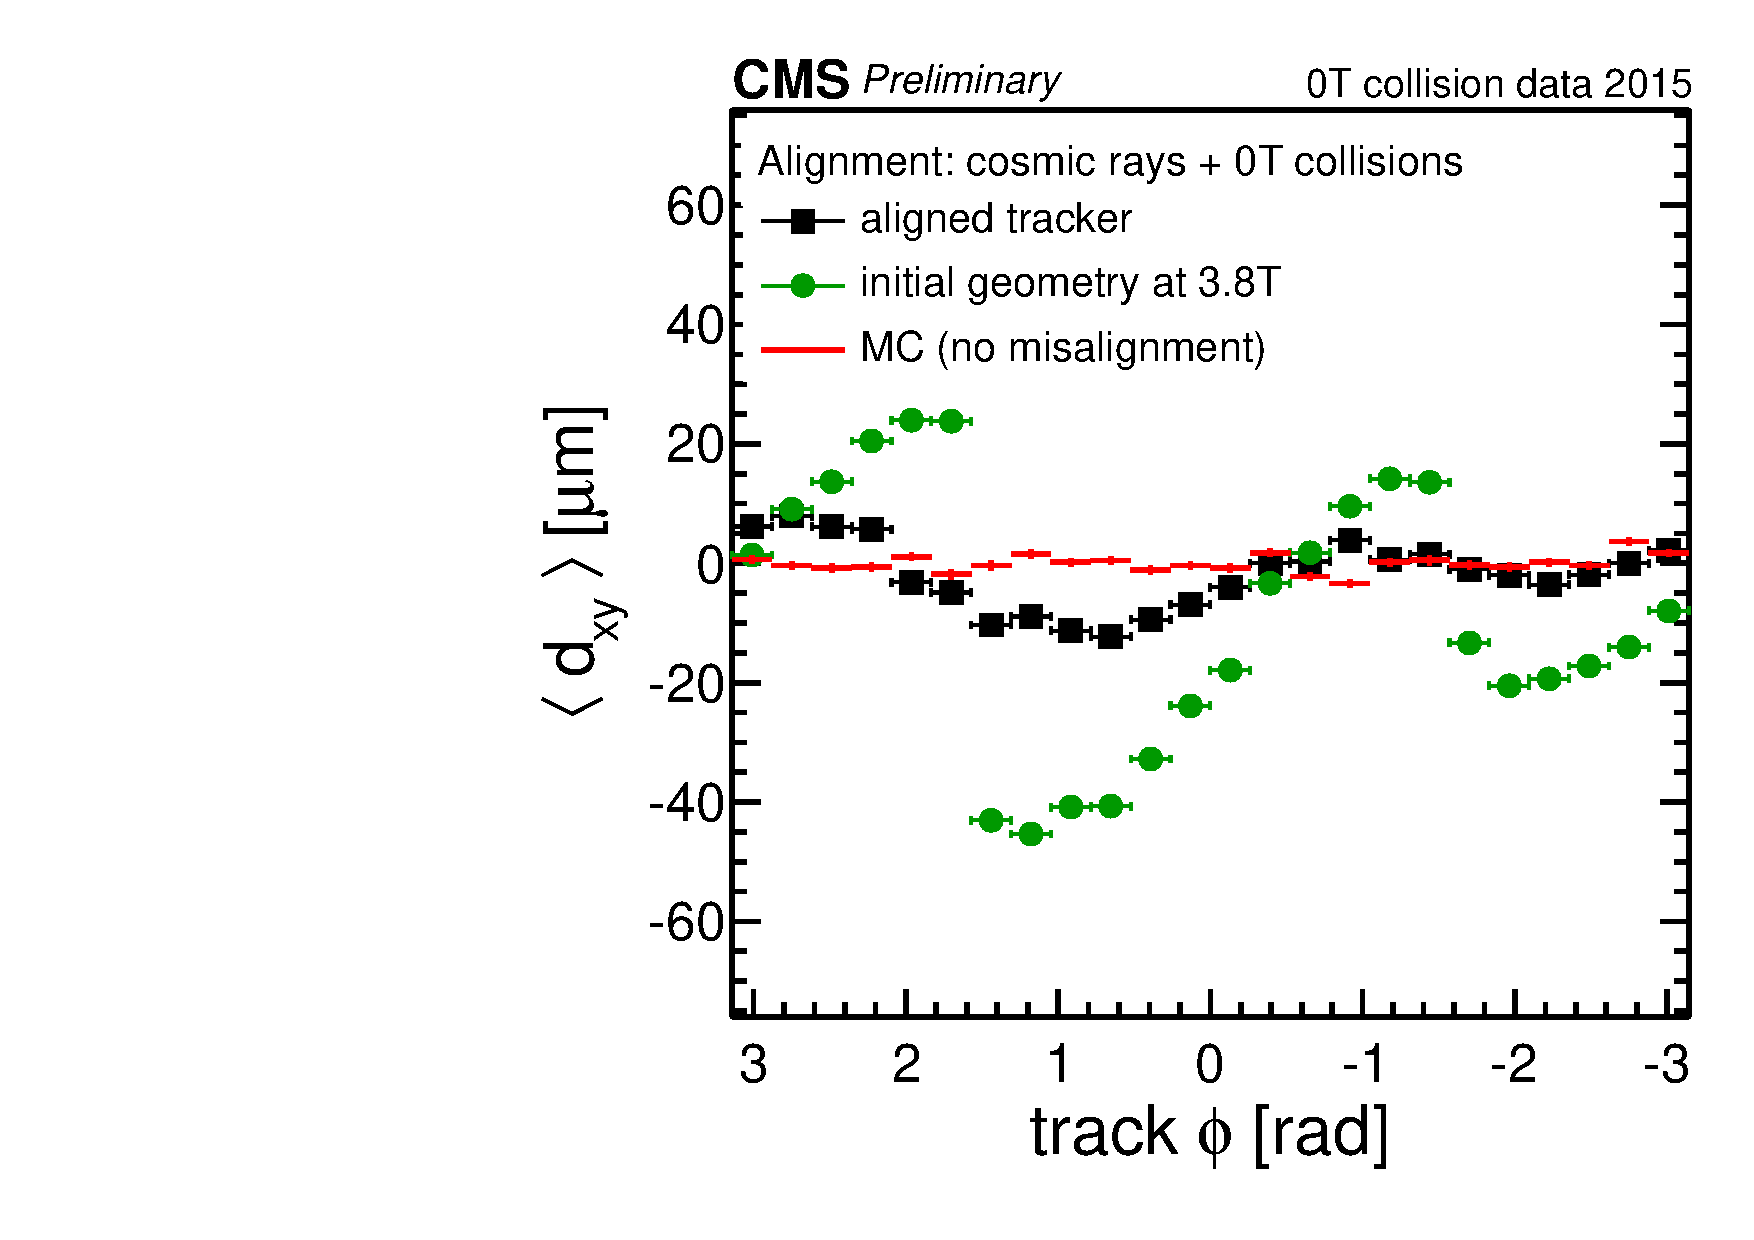
\includegraphics[width=0.45\textwidth]{../figs/Alignment/AlRes_dxyPhiBiasCanvas.pdf}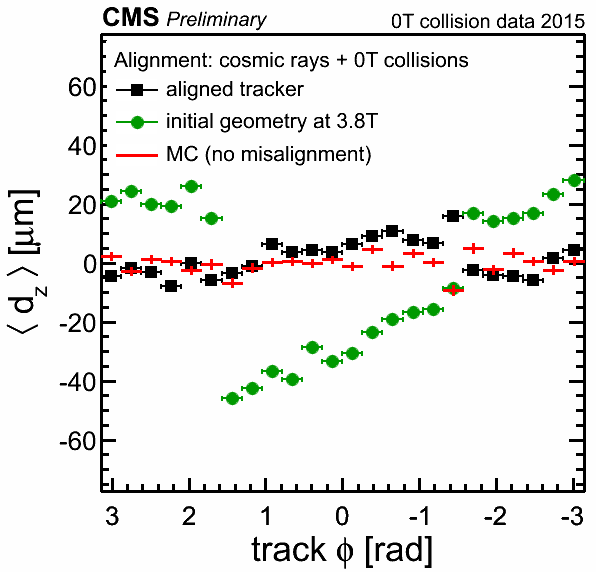
\includegraphics[width=0.45\textwidth]{../figs/Alignment/AlRes_dzPhiBiasCanvas.png}
    \end{center}
    \caption{The results of the primary vertex validation. The distance of the track at its closest approach to a refit unbiased primary vertex ($d_{xy}$, left and $d_z$, right) in the transverse plane. The validation is produced with $B=0$T collision data. The alignment is produced with the Millepede-II and HIP algorithms using ~$B=0$T and~$B=3.8$T cosmic ray data and $B=0$T collision data. }
    \label{fig:PVvalidation}
\end{figure}

%\begin{figure}[htb]
%    \begin{center}
%        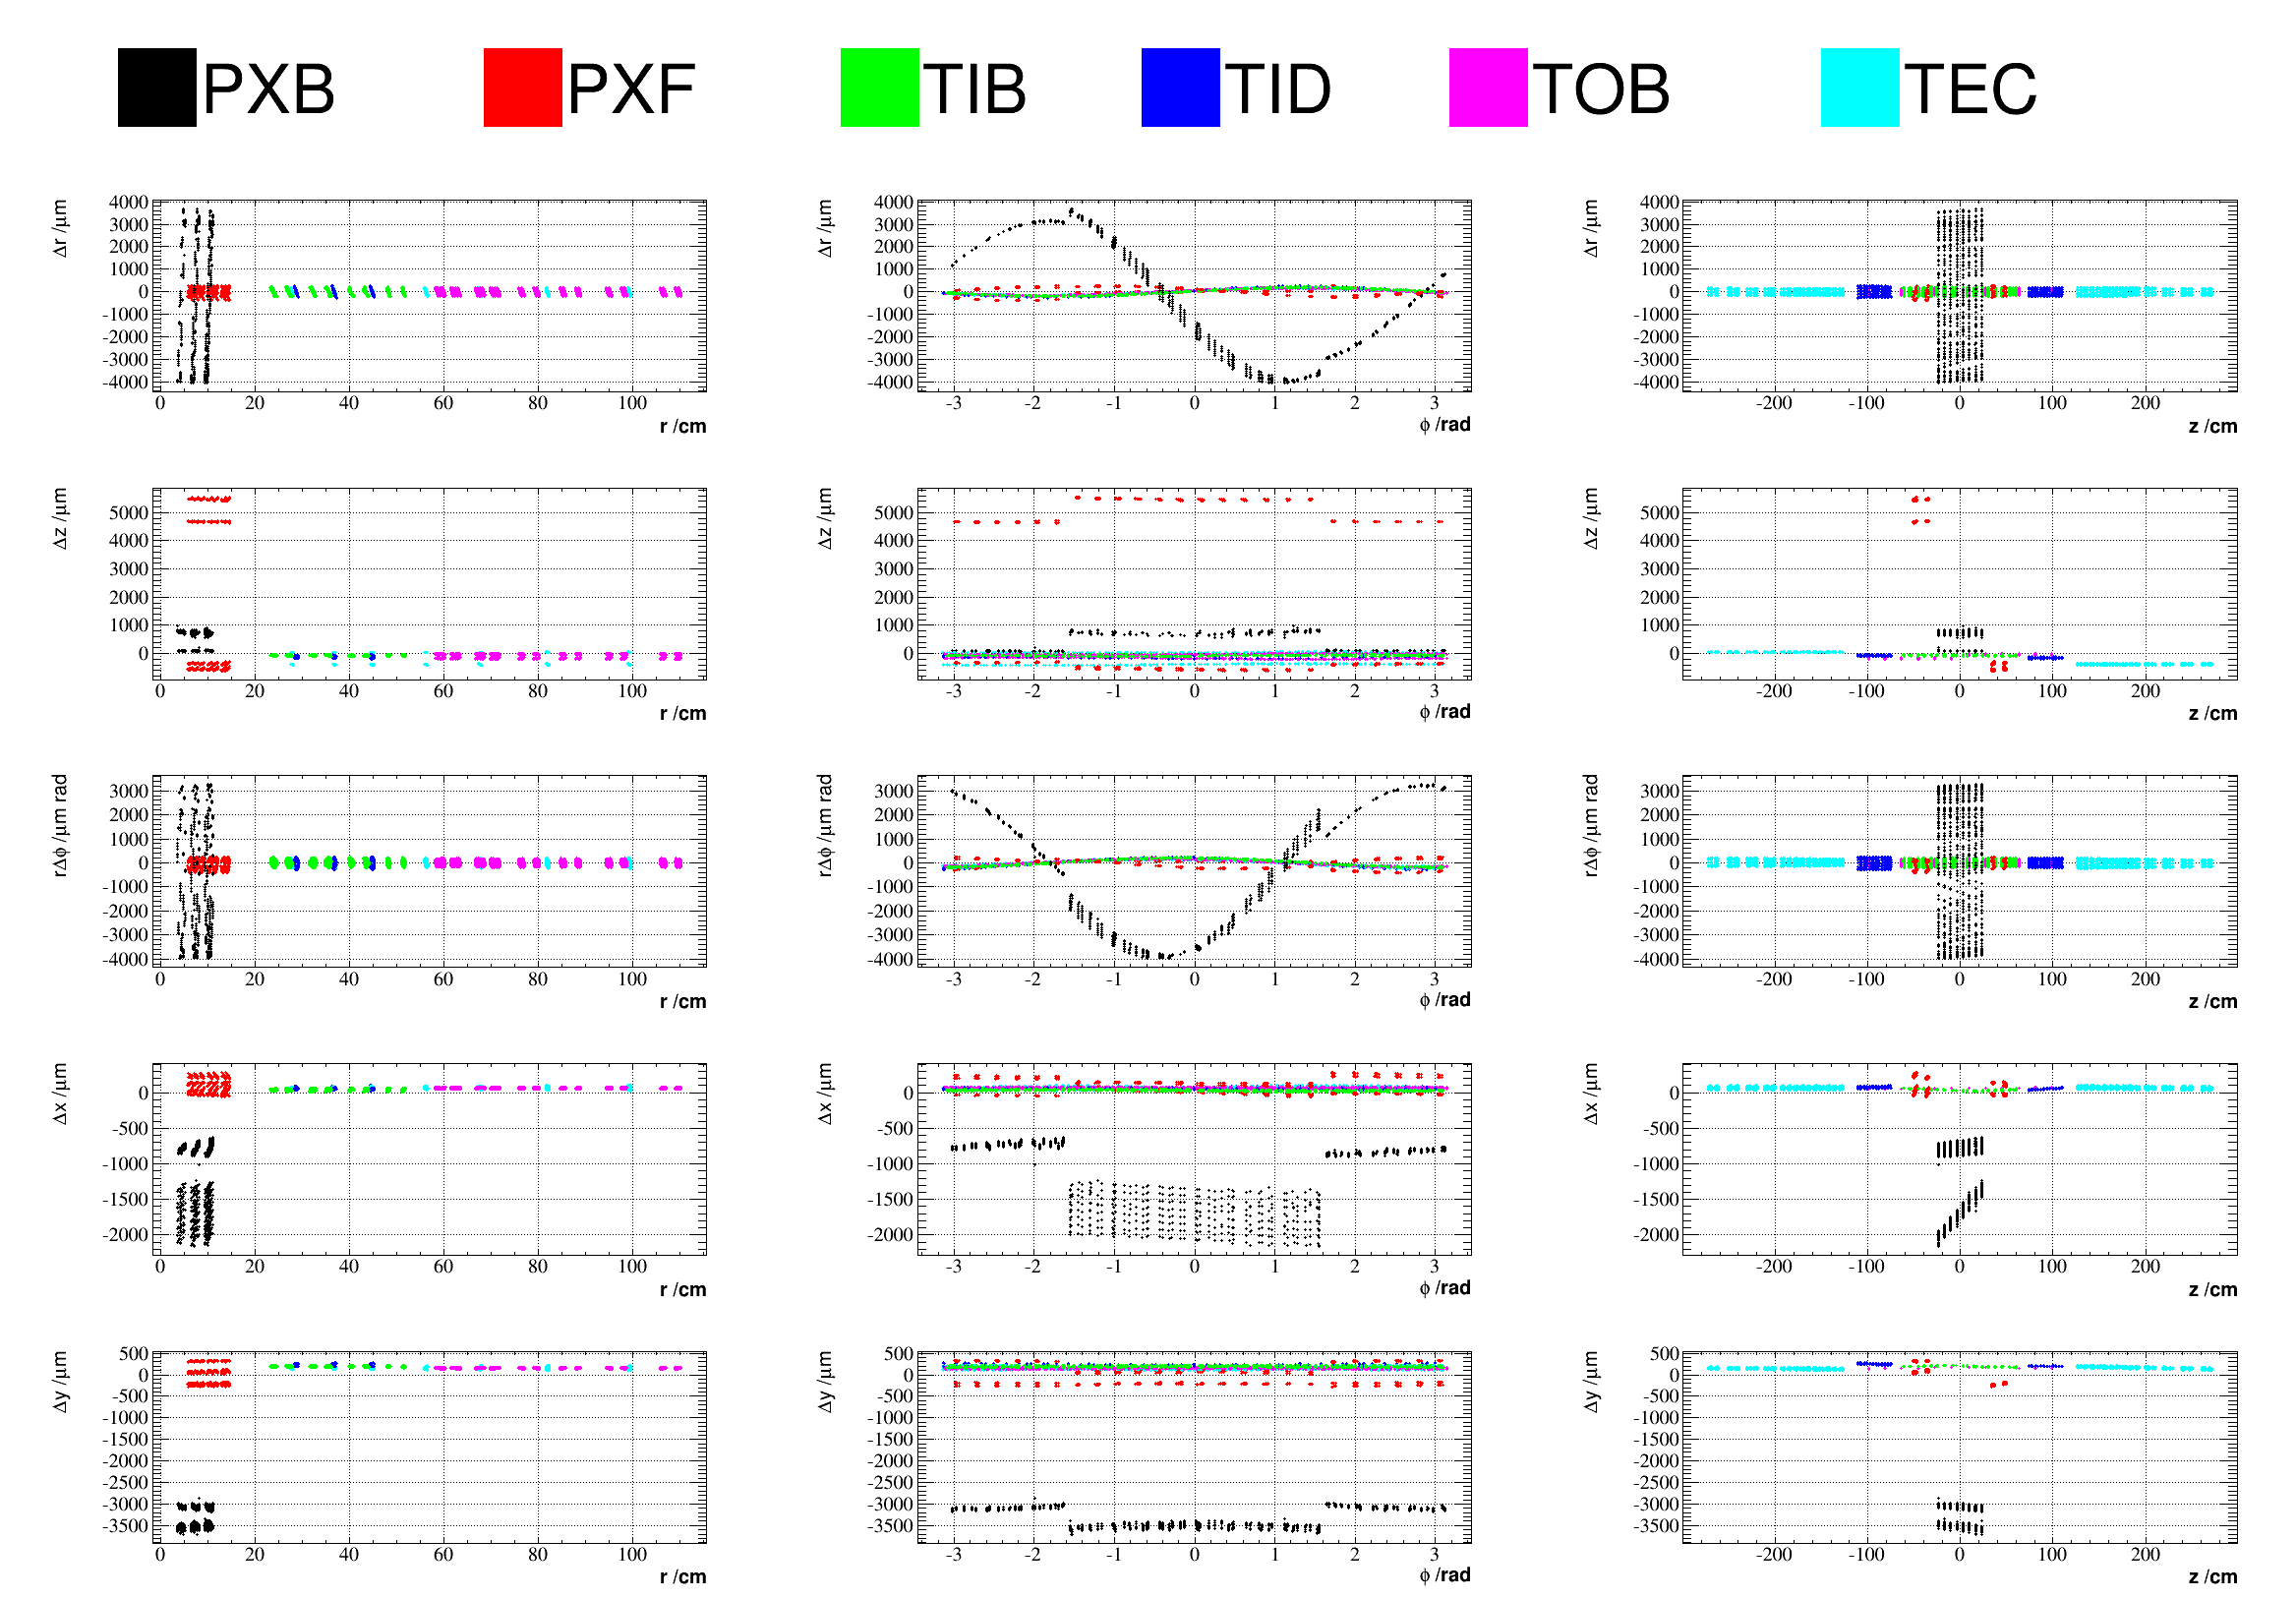
\includegraphics[width=0.98\textwidth]{../figs/Alignment/global_tracker_2_final.png}
%    \end{center}
%    \caption{Geometry comparison plot of CRUZET 2015 object vs Run I.}
%    \label{fig:trackAndResiduals}
%\end{figure}

%(12) NO PLAGIARISM DETECTED
Given the complexity of the CMS detector, any single measurement based on CMS data requires an excellent understanding of the geometry and response of all systems to particles of all types. The CMS Alignment and Calibration team coordinates hundreds of CMS physicists who are working on various aspects of this. The Chapter~\ref{sec:alignment} of this dissertation presented one aspect of this work that concerns alignment of one system of CMS, the part in which the author of this dissertation played an important role.
